%%%%%%%%%%%%%%%%%%%%%%%%%%%%%%%%%%%%%%%%%%%%%%%%%%%%%%%%%%%%%%%%%%%%%%%%%%%%%%%%%%%%%
% PACOTES                                                                           %
%%%%%%%%%%%%%%%%%%%%%%%%%%%%%%%%%%%%%%%%%%%%%%%%%%%%%%%%%%%%%%%%%%%%%%%%%%%%%%%%%%%%%
\documentclass[a4paper,12pt]{article}

%-----------------------------------------------------------------------------------%
% LAYOUT DA PÁGINA                                                                  %
%-----------------------------------------------------------------------------------%
\usepackage[top=3cm, bottom=3cm, left=2.5cm, right=2.5cm]{geometry}
%\usepackage{fancyhdr} % Permite controlar como são exibidos os cabeçalhos

%-----------------------------------------------------------------------------------%
% FORMATAÇÃO DO TEXTO                                                               %
%-----------------------------------------------------------------------------------%
\usepackage{setspace} % Permite definir o espaçamento entre linhas

%-----------------------------------------------------------------------------------%
% PACOTES DE IMAGENS                                                                %
%-----------------------------------------------------------------------------------%
\usepackage[pdftex]{graphicx}
\pdfsuppresswarningpagegroup=1 % A warning issued when several PDF images are
% imported in the same page. Mostly harmless, can be almost always supressed.
%\usepackage[pstarrows]{pict2e} % Amplia as funcionalidades do ambiente picture
\usepackage{tikz}
\usetikzlibrary{shapes, arrows, arrows.meta}

%-----------------------------------------------------------------------------------%
% PACOTES DE TABELAS                                                                %
%-----------------------------------------------------------------------------------%
\usepackage{array} % Facilita a formatação de tabelas
%\usepackage{multirow} % Permite criar células que ocupam várias linhas em uma tabela
\usepackage{longtable} % Permite criar tabelas que quebram de página

%-----------------------------------------------------------------------------------%
% PACOTES MATEMÁTICOS DE BASE                                                       %
%-----------------------------------------------------------------------------------%
\usepackage{amsfonts,amstext,amscd,bezier,amsthm,amssymb}
\usepackage[centertags]{amsmath}

%-----------------------------------------------------------------------------------%
% PACOTES DE SÍMBOLOS MATEMÁTICOS                                                   %
%-----------------------------------------------------------------------------------%
%\usepackage{mathtools} % Símbolos matemáticos extras. (ex.: \xrightharpoon)
%\usepackage[integrals]{wasysym} % Muda o estilo das integrais, além de outros
%                                 símbolos extras
%\usepackage[nice]{nicefrac} % Permite o uso de frações "melhores". Usar \nicefrac{}{}

%-----------------------------------------------------------------------------------%
% PACOTES DE FONTES MATEMÁTICAS                                                     %
%-----------------------------------------------------------------------------------%
%\usepackage{mathbbol} % Quase todos os símbolos com \mathbb
%\usepackage{bbm} % Extensão dos símbolos de \mathbb. Usar comando \mathbbm
%\usepackage{calrsfs} % Muda o estilo de \mathcal
%\usepackage[mathcal]{euscript} % Muda o estilo de \mathcal

%-----------------------------------------------------------------------------------%
% PACOTES DE CODIFICAÇÃO DE FONTES                                                  %
%-----------------------------------------------------------------------------------%
\usepackage[utf8]{inputenc} % Permite o uso de caracteres ISO 8859-1, incluindo os
%                               caracteres acentuados diretamente.
\usepackage[T1]{fontenc} % Uso de fontes T1, necessário para tratar caracteres
%                          acentuados como um único bloco.

%-----------------------------------------------------------------------------------%
% PACOTES DE LÍNGUAS                                                                %
%-----------------------------------------------------------------------------------%
\usepackage[french]{babel} % Seleciona a língua do documento, definindo nomes de
%                              seções, nome do índice, da bibliografia, etc. Em caso
%                              de documento com mais de uma língua, a padrão é a
%                              última.
\NoAutoSpaceBeforeFDP % Utilizar em francês se quiser evitar espaços antes de :

%-----------------------------------------------------------------------------------%
% PACOTES DE BIBLIOGRAFIA                                                           %
%-----------------------------------------------------------------------------------%
%\usepackage{babelbib} % Permite definir a língua das entradas da bibliografia. Usar
%                       [fixlanguage] para uma mesma língua para todas as entradas e
%                       \selectbiblanguage{} para definir a língua. Um estilo compa-
%                       tível com babelbib deve ser usado (ex: babplain)
\usepackage{cite} % Organiza os elementos citados dentro de um mesmo \cite.

%-----------------------------------------------------------------------------------%
% PACOTES DE FONTES                                                                 %
%-----------------------------------------------------------------------------------%
% Computer Modern (fonte padrão)                                                    %
% - - - - - - - - - - - - - - - - - - - - - - - - - - - - - - - - - - - - - - - - - %
%\usepackage{ae} % A usar com a fonte padrão do LaTeX quando forem gerados PDFs, para
%                 corrigir erros de visualização

% Computer Modern Bright (sans serif)                                               %
% - - - - - - - - - - - - - - - - - - - - - - - - - - - - - - - - - - - - - - - - - %
%\usepackage{cmbright}

% Times New Roman                                                                   %
% - - - - - - - - - - - - - - - - - - - - - - - - - - - - - - - - - - - - - - - - - %
%\usepackage{mathptmx} % Muda texto e modo matemático
%\usepackage{times} % Apenas texto, não muda modo matemático

% Arial                                                                             %
% - - - - - - - - - - - - - - - - - - - - - - - - - - - - - - - - - - - - - - - - - %
%\usepackage[scaled]{uarial} % Arial como fonte sans serif padrão

% Palatino                                                                          %
% - - - - - - - - - - - - - - - - - - - - - - - - - - - - - - - - - - - - - - - - - %
%\usepackage{mathpazo} % Muda texto e modo matemático
%\usepackage{palatino} % Apenas texto, não muda modo matemático

% Concrete                                                                          %
% - - - - - - - - - - - - - - - - - - - - - - - - - - - - - - - - - - - - - - - - - %
%\usepackage{ccfonts} % Texto: Concrete; Matemático: Concrete Math
%\usepackage{ccfonts, eulervm} % Texto: Concrete; Matemático: Euler

% Iwona                                                                             %
% - - - - - - - - - - - - - - - - - - - - - - - - - - - - - - - - - - - - - - - - - %
%\usepackage[math]{iwona} % Texto e modo matemático: Iwona

% Kurier                                                                            %
% - - - - - - - - - - - - - - - - - - - - - - - - - - - - - - - - - - - - - - - - - %
%\usepackage[math]{kurier} % Texto e modo matemático: Kurier

% Antykwa Póltawskiego                                                              %
% - - - - - - - - - - - - - - - - - - - - - - - - - - - - - - - - - - - - - - - - - %
%\usepackage{antpolt} % Texto: Antykwa Póltawskiego; Matemático: nenhum
                     % Usar fontenc = QX ou OT4

% Utopia                                                                            %
% - - - - - - - - - - - - - - - - - - - - - - - - - - - - - - - - - - - - - - - - - %                     
%\usepackage{fourier} % Texto: Utopia; Matemático: Fourier

% KP Serif                                                                          %
% - - - - - - - - - - - - - - - - - - - - - - - - - - - - - - - - - - - - - - - - - %
\usepackage{kpfonts}

%-----------------------------------------------------------------------------------%
% CORES                                                                             %
%-----------------------------------------------------------------------------------%
\usepackage{color}
\definecolor{darkgreen}{rgb}{0,0.5,0}
\definecolor{darkmagenta}{rgb}{0.5,0,0.5}
\definecolor{darkgray}{rgb}{0.5,0.5,0.5}
\definecolor{darkblue}{rgb}{0.2,0.2,0.4}
\definecolor{darkred}{rgb}{0.6,0.15,0.15}
\definecolor{gray}{rgb}{0.65,0.65,0.65}
\definecolor{lightgray}{rgb}{0.8,0.8,0.8}
\definecolor{lightblue}{rgb}{0.5,0.5,1}
\definecolor{lightgreen}{rgb}{0.5,1,0.5}
\definecolor{deadred}{rgb}{0.7, 0.2, 0.2}
\definecolor{deadblue}{rgb}{0.2, 0.2, 0.7}

%-----------------------------------------------------------------------------------%
% PACOTES DIVERSOS                                                                  %
%-----------------------------------------------------------------------------------%
\usepackage{icomma} % Permite uso de vírgula como separador decimal
\usepackage{url} % Pacote para não ter problemas com URLs. Usar \url{}
%\usepackage{randtext} % Troca a ordem de letras de uma frase (útil com e-mails em
                      % PDFs a serem publicados on-line.
\usepackage[hidelinks]{hyperref}
%\usepackage{showkeys} % Para mostrar o nome dos labels
\usepackage{enumitem} % Facilita o uso de listas, inclusive referências a itens de
                      % listas.
%\usepackage[absolute]{textpos} % Posição absoluta de texto na página
%\usepackage{pdfpages} % Permite incluir documentos em PDF no arquivo
%\usepackage{refcheck} % Verifica as referências procurando por
%                      % labels não usados ou equações numeradas sem labels.
%                      % Verificar o arquivo .log e procurar por RefCheck.
%\usepackage[french]{algorithm2e}

%%%%%%%%%%%%%%%%%%%%%%%%%%%%%%%%%%%%%%%%%%%%%%%%%%%%%%%%%%%%%%%%%%%%%%%%%%%%%%%%%%%%%
% CONFIGURAÇÕES                                                                     %
%%%%%%%%%%%%%%%%%%%%%%%%%%%%%%%%%%%%%%%%%%%%%%%%%%%%%%%%%%%%%%%%%%%%%%%%%%%%%%%%%%%%%

%-----------------------------------------------------------------------------------%
% FORMATAÇÃO DO TEXTO                                                               %
%-----------------------------------------------------------------------------------%
%\onehalfspacing % Espaçamento 1 1/2 (definido no pacote setspace)
\setstretch{1.1}
\setlength{\parskip}{6pt plus 2pt minus 1pt}
%-----------------------------------------------------------------------------------%
% DEFINIÇÃO DE AMBIENTES MATEMÁTICOS                                                %
%-----------------------------------------------------------------------------------%
%\theoremstyle{plain}
%\newtheorem{theo}{Teorema}[section]
%\newtheorem{lemm}[theo]{Lema}
%\newtheorem{coro}[theo]{Corolário}
%\newtheorem{prop}[theo]{Proposição}
%\theoremstyle{definition}
%\newtheorem{defi}[theo]{Definição}
%\newtheorem{remq}[theo]{Observação}
%%\newtheorem{expl}[theo]{Exemplo}
%\newenvironment{expl}%
%  {\refstepcounter{theo}%
%    \begin{list}{}{%
%    \setlength{\topsep}{0pt}%
%    \setlength{\leftmargin}{\parindent}%
%    \setlength{\rightmargin}{0pt}%
%    \setlength{\listparindent}{\parindent}%
%    \setlength{\itemindent}{0pt}%
%    \setlength{\parsep}{\parskip}}%
%    \item[]{\bf Exemplo \thetheo. }}%
%  {\hspace*{\fill} $\square$ \end{list} \medskip}
%\newenvironment{solu}%
%  {\noindent {\bf Solução. }\small}%
%  {\hspace*{\fill} $\square$ \normalsize \medskip}
%\newenvironment{dems}[1][Demonstração]%
%  {\begin{list}{}{%
%    \setlength{\topsep}{0pt}%
%    \setlength{\leftmargin}{\parindent}%
%    \setlength{\rightmargin}{0pt}%
%    \setlength{\listparindent}{\parindent}%
%    \setlength{\itemindent}{0pt}%
%    \setlength{\parsep}{\parskip}}%
%    \item[]{\bf #1. }}%
%  {\hspace*{\fill} $\blacksquare$ \end{list} \medskip}


%-----------------------------------------------------------------------------------%
% DEFINIÇÃO DE COMANDOS MATEMÁTICOS                                                 %
%-----------------------------------------------------------------------------------%
%\newcommand*\diff{\mathop{}\!\mathrm{d}}

%\newcommand{\norm}[1]{\left\lVert #1\right\lVert} % Norma
%\newcommand{\abs}[1]{\left\lvert #1\right \rvert} % Valor absoluto
%\newcommand{\floor}[1]{\left\lfloor #1 \right\rfloor} % Arredondar para baixo
%\newcommand{\ceil}[1]{\left\lceil #1 \right\rceil} % Arredondar para cima


%-----------------------------------------------------------------------------------%
% NUMERAÇÃO DE ELEMENTOS                                                            %
%-----------------------------------------------------------------------------------%
%\numberwithin{table}{section}
%\numberwithin{table}{subsection}
%\numberwithin{figure}{section}
%\numberwithin{figure}{subsection}
\numberwithin{equation}{section}
%\numberwithin{equation}{subsection}
%\numberwithin{theo}{chapter}
%\numberwithin{theo}{subsection}

%%%%%%%%%%%%%%%%%%%%%%%%%%%%%%%%%%%%%%%%%%%%%%%%%%%%%%%%%%%%%%%%%%%%%%%%%%%%%%%%%%%%%
% ESTRUTURA DO DOCUMENTO                                                            %
%%%%%%%%%%%%%%%%%%%%%%%%%%%%%%%%%%%%%%%%%%%%%%%%%%%%%%%%%%%%%%%%%%%%%%%%%%%%%%%%%%%%%
\begin{document}

\title{2I013 Projet \\ Groupe 1 : Football et stratégie}
\author{Ariana Carnielli et Parth Shah}
\date{}

\maketitle

\tableofcontents
\newpage

\section{Introduction}

Ce projet s’intéresse à la programmation des stratégies pour l’automatisation des joueurs dans le jeu de  « football » SoccerSimulator (disponible sur \url{https://github.com/baskiotisn/SoccerSimulator-2017}). Il s'agit d'un jeu codé en Python où les joueurs peuvent s’affronter dans plusieurs types de matchs : en 1 contre 1, en 2 contre 2 ou encore en 4 contre 4. Les joueurs et la balle peuvent se déplacer partout sur un terrain de jeu dont la taille est fixée par deux constantes et est constitué de deux cages placés aux bords verticaux. Si la balle touche les bords du terrain, elle rebondit, par contre les joueurs ne rebondissent pas et perdent toute leurs vitesses. Les joueurs ne sont pas considérés comme des obstacles à la balle, celle-ci peut les croiser sans rebondir. Chaque match est joué en temps discret, donné aussi par une constante. À chaque pas de temps le jeu actualise la position de chaque objet mobile sur le terrain et vérifie si un but a été marqué. Dans ce cas, les positions des joueurs et de la balle sont réinitialisées. Le jeu se joue de manière autonome, chaque joueur choisissant une action à chaque pas de temps en accord à la stratégie qui lui a été passée.

L’objectif est d’implémenter des stratégies permettant à nos joueurs de gagner la plus grande quantité de matchs contre les stratégies adverses codés par d'autres binômes. Dans ce rapport, nous présentons la démarche mise au point lors de la conception des stratégies tout en abordant les problèmes rencontrés. Dans un second temps nous exposons des stratégies que nous avons écrites et l'implémentation de l’algorithme génétique pour leur optimisation ainsi que l’implémentation des arbres de décision. Une conclusion récapitule les principaux points de ce rapport et les compétences acquises.

\section{Démarche utilisée et problèmes rencontrés}

Pour construire des stratégies, plusieurs classes étaient à notre disposition, notamment \texttt{SoccerAction}, \texttt{Vector2D} et \texttt{SoccerState}. \texttt{Vector2D} contient deux coordonnées \texttt{x} et \texttt{y} ainsi que de méthodes pour, par exemple, calculer la norme d’un vecteur donné et son angle par rapport aux axes des coordonnés. Quant à \texttt{SoccerAction}, celui-ci est composé de deux \texttt{Vector2D} : un qui donne la direction du mouvement du joueur et un autre qui donne la direction du shoot. \texttt{SoccerState} contient toutes les informations nécessaires pour connaitre l’état du jeu à un moment donné y compris la position et vitesse de la balle et de tous les joueurs. 

Il existe déjà une classe \texttt{Strategy} donnant la base pour la construction d'une stratégie : Toute classe de stratégie que nous avons codé hérite de celle-ci. Une stratégie doit implémenter une méthode \texttt{compute\_strategy} qui prend en argument l'état du jeu à travers un \texttt{SoccerState} et l'identification d'un joueur et retourne un \texttt{SoccerAction} à chaque pas de temps. Au départ nos stratégies étaient des classes indépendantes regroupés dans un fichier appelé \texttt{strategy.py}.
	
Comme nous n’avions aucune expérience sur la conception de stratégies, nous avons tout d’abord essayé de coder une petite stratégie telle qu’un fonceur, en reprenant l’exemple vu en cours, qui court vers la balle et tire au but. Notre intention était de l’utiliser principalement en 1 contre 1. Nous nous sommes rendu compte après quelques essais qu’il serait intéressant de ne pas encombrer la stratégie avec des tests pour voir si le joueur a la balle, etc., car à chaque fois que nous voulions changer un paramètre ou les choix faits par la stratégie, il fallait changer tout le code. Nous avons ainsi crée une classe appelée \texttt{ToolBox} avec des méthodes qui retournaient les résultats des tests fréquents qu’on utilisait, dans un fichier nommé \texttt{toolbox.py}.

Au fur et à mesure du projet nous étions amenés à développer de nombreuses stratégies et nous avons remarqué que plusieurs d'entre elles partageaient des morceaux de code suffisamment complexes pour ne pas être dans \texttt{ToolBox}. Nous avons alors rajouté de couches entre nos stratégies et \texttt{ToolBox} en créant d'autres classes. Cela a permis également de rendre le code plus lisible et modulaire. Nous avons mis au point deux fichiers en plus de \texttt{toolbox.py} : \texttt{action.py} et \texttt{comportement.py}. Ainsi, en cas de problème à l’exécution, nous pouvions le trouver plus facilement et modifier seulement la partie de la fonction ou méthode concernée, plutôt que l’intégralité du code.

Nous avons décidé de laisser \texttt{ToolBox} avec toutes les méthodes retournant des booléens, des \texttt{Vector2D} et des listes de \texttt{Vector2D}. Les fichiers \texttt{action.py} et \texttt{comportement.py} ont chacun une classe homonyme : \texttt{Action} contient des méthodes qui retournent des \texttt{SoccerAction} alors que \texttt{Comportement} utilise les méthodes dans \texttt{ToolBox} et \texttt{Action} pour bien choisir le \texttt{SoccerAction} qu'une stratégie doit retourner à chaque pas de temps. Nous avons choisi de séparer les comportements des stratégies afin d’être capable d’appeler plusieurs comportements dans une stratégie quelconque. À la fin, nous avons trouvé cela un peu redondant car nos stratégies appellent uniquement un comportement même si le fait de séparer stratégie et comportement a été utile dans une stratégie décrite plus en détail dans la section suivant.

Tous nos fichiers ont été mis dans un même module contenant un fichier principal \texttt{\_\_init\_\_.py}, où la fonction de création de joueurs en appelant nos stratégies a été placée. Pour ce faire, nous avons eu besoin de la commande \texttt{import} de Python pour l'utilisation d’une classe ou bien d’une fonction écrite dans un autre fichier. Au début, lorsque nous lancions notre fichier exécutable, quelques erreurs apparaissaient à cause des \texttt{import} non aboutis. En effet, la syntaxe de \texttt{import} en Python change selon la version du langage et si l'importation est absolue ou relative. Nous avons donc utilisé exclusivement Python 3, qui utilise des import relatifs explicites, pour régler les soucis.

Nous nous sommes mis à développer également d’autres stratégies plus intéressantes qu’un fonceur, notamment des défenseurs et des dribleurs. Le développement continu de ces stratégies était indispensable pour contrer les améliorations apportées par les autres binômes à leurs stratégies, afin de permettre ainsi une bonne cohésion entre nos joueurs et un équilibre entre la quantité de buts marqués et encaissés pour enfin obtenir un bon rang dans les classements. La section suivante présentera plus en détails nos principales stratégies, leur fonctionnement et les raisonnements derrière nos choix.

Après quelques séances nous nous sommes rendu compte que la meilleure façon de battre tous nos adversaires était d’étudier plus en détail chacune de leurs stratégies et d’en exploiter les faiblesses afin d'avoir l’avantage. C’est pourquoi nous avons commencé à télécharger les modules des autres binômes depuis leurs dossiers en ligne sur \emph{Github}. Pour chaque groupe, nous essayions d’améliorer et de réajuster notre code en fonction des résultats obtenus en simulant des matchs pour enfin arriver à une moyenne de victoires convenable. 

En revanche, il n’était pas toujours facile de trouver une riposte contre les stratégies des autres groupes. Certaines stratégies étaient si bien codées qu’il fallait du temps pour d’abord mettre au point de nouvelles stratégies pour contrer une attaque ou intercepter la balle par exemple, d’autant plus que ces tests devaient être réalisés contre l’ensemble des autres binômes. En outre, certaines étaient mises en ligne quelques instants avant les résultats finaux, nous empêchant ainsi de pouvoir travailler sur les stratégies récentes. En utilisant la recherche exhaustive et l'algorithme génétique nous avons enfin automatisé une partie du processus d’amélioration de nos stratégies, dont la démarche sera présenté dans la Section \ref{4}.

\section{Présentation des stratégies}

Cette section présente les principales \og familles \fg{} de stratégies que nous avons codées à la main pour ce projet : Fonceur, Dribbleur, Défenseur et Attaquant. Cette division suit l'évolution de notre code dans le sens où le Fonceur et ses améliorations ont été les premières stratégies codées, suivies par le Dribleur et le Défenseur qui nous ont permis de passer aux matchs 2 contre 2 et enfin l'Attaquant qui a été crée pour les matchs 4 contre 4.   

\subsection{Fonceur}

Comme nous avons dit précédemment, la première stratégie codée a été le Fonceur qui peut être représenté par l'arbre de décision de la Figure \ref{Figure1}.

\begin{figure}[ht]
\centering
\tikzstyle{block} = [rectangle, rounded corners=3mm, very thick, font=\small, draw=blue!50!white, fill=blue!10!white]
\tikzstyle{decision} = [diamond, rounded corners=3mm, shape aspect=2.5, very thick, font=\small, draw=red!50!white, fill=red!10!white, inner sep=0mm]

\begin{tikzpicture}

\node[decision] (test1) at (0, 0) {\parbox[c][\height][c]{4cm}{\centering Peut tirer? }};
\node[block, anchor = north] (oui) at (-3, -2) {\parbox[c][\height][c]{4cm}{\centering Tirer vers le centre du but}};
\node[block, anchor = north] (non) at (3, -2) {\parbox[c][\height][c]{4cm}{\centering Courir vers le ballon}};
\draw[thick, -Stealth] (test1) -- node[midway, above left]{\small Oui} (oui);
\draw[thick, -Stealth] (test1) -- node[midway, above right]{\small Non} (non);

\end{tikzpicture}
\caption{Arbre de décision du Fonceur}
\label{Figure1}
\end{figure}

Dans un premier temps cette stratégie a été code sans aucune paramètre mais nous avons ensuite identifié quelques uns ayant une influence sur le comportement et l’efficacité de cette stratégie : l’accélération du joueur quand il court, l'accélération de son tir et la quantité de pas de temps en avance qu'il essaie de prévoir la position du ballon.

Lorsque ce fonceur joue contre d'autres stratégies de fonceur identiques ou très similaires, il arrive assez souvent qu'on tombe sur une situation de \og blocage \fg, où les deux joueurs courent ensemble vers le ballon, arrivant et tirant au même moment en directions opposées, auquel cas le ballon part dans un direction essentiellement aléatoire et aucun des deux joueurs n'arrive à marquer un but. Ce blocage peut être partiellement résolu en changeant le nombre de pas de temps de prévision de la position du ballon, mais cette solution ne donne pas en général des résultats satisfactoires, surtout car une quantité de pas de temps peut être très bonne pour certaines variantes du fonceur, mais pas pour d'autres. Cela nous a motivés à créer une stratégie plus élaborée, le Dribbleur, décrit dans la prochaine partie.

\subsection{Dribbleur}

\noindent \textcolor{red}{\rule{\textwidth}{0.5cm}}

Finalement, la stratégie qui forme la pièce maitresse de notre jeu est le dribbleur. La dernière prend en paramètre la vitesse v, le nombre d’étapes n, l’accélération pour faire un tir mais aussi pour dribbler. Il est nécessaire que le joueur dribble à une vitesse optimale pour qu’il soit assez rapide afin de se déplacer sur l’ensemble du terrain tout en contournant ses adversaires. Il prend également un angle qui va nous servir à déterminer la direction du tir en fonction de l’adversaire. Ce dribbleur est utile pour favoriser la liaison entre la défense et l’attaque et contrairement aux stratégies précédentes, il est autonome c’est-à-dire qu’il ne dépend pas de ses co-équipiers mais uniquement de ses adversaires, c’est pourquoi nous pouvons l’utiliser dans tous les types de matchs : en 1 contre 1, en 2 contre 2 voire en 4 contre 4…
	
Ainsi, le programme détermine d’emblée s’il le joueur est à proximité de la balle puis calcule la position cette fois de l’adversaire le plus proche de lui, pour remonter progressivement vers les cages de l’équipe adverse. Il calcule ensuite l’angle entre lui et l’adversaire : si l’adversaire est situé en bas par rapport au joueur, il dribble vers le haut, et au contraire si l’adversaire est situé en haut par rapport au joueur, il dribble vers le bas. Lorsqu’il n’y a plus aucun adversaire en face de lui, il finit par marquer un but. En revanche, s’il n’est pas en mesure de dribbler, il court vers la balle pour exécuter les dernières instructions.

\noindent \textcolor{red}{\rule{\textwidth}{0.5cm}}

Parmi les stratégies que nous avons codées, il y a celle du gardien appelée GardienStrat. Celle-ci prend en paramètre l’accélération a, la vitesse v, le nombre d’étapes n et enfin la variable p qui désigne la position pour la coordonnée x de la cage de défense. Notre but était de nous s’assurer que lorsqu’un attaquant de l’équipe adverse s’attaque à notre gardien, ce dernier puisse le confronter et adopte un certain comportement, empêchant ainsi aux ennemis de marquer un but. 

Pour ce faire, nous avons mis en place un programme qui vérifie d’abord si le gardien est à proximité du ballon. Si tel est le cas, le gardien va dégager la balle pour permettre aux autres joueurs de l’intercepter. Puis il calcule si le ballon se trouvera dans la cage de défense dans n étapes pour ensuite courir vers la position attendue si besoin, afin de s’emparer de la balle. Enfin, on vérifie si le gardien est bien positionné dans le champ défensif et si ce n’est pas le cas, il court vers sa cage pour éviter qu’un ennemi profite de l’occasion pour marquer un but.

Par ailleurs, nous avons également codé un défenseur, nommé DefStrat qui possède certains comportements similaires à notre gardien, leurs objectifs communs étant le même : celui de défendre. En plus des paramètres du gardien, il prend une variable frac\_p qui est une position défensive d’interception. Son but consistait principalement à empêcher le jeu d'attaque de l'équipe adverse.

Ainsi, le programme créé vérifie d’abord si le défenseur est à proximité du ballon. Si cette condition est remplie, le défenseur va dégager la balle pour continuer le jeu. Ensuite il détermine si le ballon se trouvera dans la cage de défense dans n étapes dans le but de courir vers la position attendue. Si ces conditions ne sont pas respectées, le défenseur court vers une position pour intercepter la balle pour ensuite la passer aux attaquants.

D’autre part, nous avons codé une stratégie de passe entre les joueurs appelée PassStrat.
Cette stratégie prend en paramètre deux accélérations différentes : une pour tirer et une autre pour faire la passe. Nous avons créé la dernière pour que la passe ne soit ni trop longue ni trop courte pour favoriser l’avancement progressif de la balle entre les joueurs jusqu’aux attaquants. En plus de l’accélération, elle prend en paramètre la vitesse et le nombre d’étapes.

Le programme se charge de d’abord déterminer si le joueur est à proximité du ballon, puis calcule la position du joueur qui est le plus proche de lui car il est inutile de faire une passe à un joueur qui est loin, les adversaires pouvant intercepter la balle et prendre le jeu à leur avantage. Une fois la position calculée, il fait la passe à ce joueur, sinon il fait une passe au gardien. Enfin, s’il n’est pas proche de ballon, il court vers celui-ci pour ensuite faire les instructions ci-dessus.



\section{Optimisation des stratégies}
\label{4}


\subsection{Recherche exhaustive}

Pour le chalenge consistant à faire le nombre maximal de buts en 10000 pas de temps (sans joueur adverse), nous avons utilisé ce Fonceur sans prévision de la position du ballon et avec accélération de course maximale mais avec optimisation de l'accélération de tir. Cette optimisation a été faite par une recherche exhaustive en discrétisant l’intervalle d'accélérations possibles et cherchant à minimiser le temps nécessaire pour marquer 10 buts. Comme celle-ci a été fait avant la partie du cours sur la recherche exhaustive, nous avons dû coder par nous mêmes tous les fonctions nécessaires. Le résultat de cette optimisation est présenté dans la Figure \ref{Figure2}. 

\begin{figure}[ht]
\centering
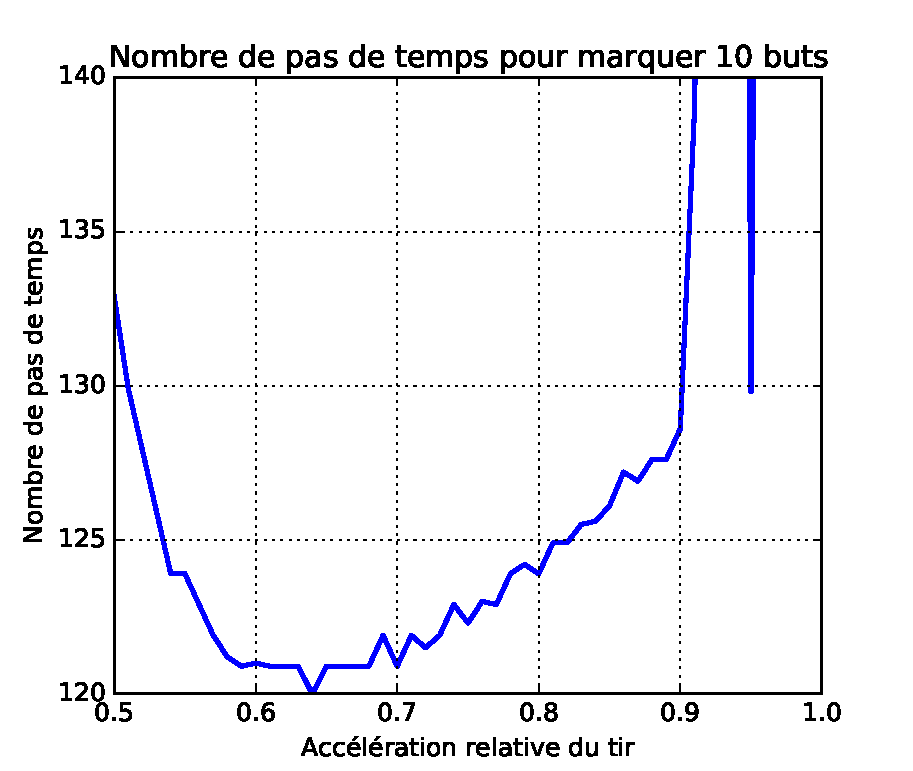
\includegraphics[scale = 0.67]{param_search_chalenge}
\caption{Recherche exhaustive de l'accélération de tir optimale}
\label{Figure2}
\end{figure}

L'accélération est donné en fraction de l'accélération maximale d'un tir. Nous pouvons voir sur la figure que sa valeur optimale est 0.64. En réalisant de simulations nous avons pu constater que, avec cette accélération, 2 tirs sont nécessaires pour marquer un but. Nous avons donc codé une recherche exhaustive sur 2 paramètres (correspondant chacun à l’accélération d'un tir) mais le résultat était que 2 tirs de la même intensité étaient l'optimum. Par contre, la accélération optimale pour cette chalenge n'est pas bonne pour les matchs.


\subsection{Algorithme génétique}

\subsection{Arbres de décision}



\section{Conclusion}

Ce projet a été l’occasion de s’intéresser au développement de stratégies en Python, et à comprendre certains principes sur le Football. Je pense que c’est un thème qu’il faut étudier, et que très peu de personnes connaissent. La réalisation des expériences nous a permis de comprendre les difficultés du projet en soi, notamment avec la prise en main de Github, à repenser aux stratégies qu’il faut utiliser… Mais au-delà d’un grand apport de connaissances, le projet a été l’opportunité de chercher seules des solutions à nos problèmes. Le travail d’équipe a, je pense aussi nouer des liens entre nous. Nous avons fait d’énormes progrès en informatique, en particulier avec la programmation en Python, à travers les stratégies.

\end{document}
